\documentclass[aspectratio=169,11pt]{beamer}
\usepackage{teaching_slides}

\title{Multinomial Discrete Choice: IIA Logit}
\author{Chris Conlon}
\institute{Grad IO}
\date{Fall 2026}

\begin{document}
\frame{\titlepage}


\begin{frame}
\frametitle{Motivation}
Most decisions agents make are not necessarily binary:
\begin{itemize}
\item Choosing a level of schooling (or a major).
\item Choosing an occupation.
\item Choosing a partner.
\item Choosing where to live.
\item Choosing a brand of (yogurt, laundry detergent, orange juice, cars, etc.).
 \end{itemize}
\end{frame}

\begin{frame}
\frametitle{Nonparametric Setup}
We consider a \alert{multinomial discrete choice}:
\begin{itemize}
\item in period $t$
\item with $\calJ_t$ alternatives.
\item subscript individual agents by $i$.
\item agents choose $j \in J_t$ with probability $\sigma_{ijt}$.
\item Agent $i$ receives utility $U_{ijt}$ for choosing $j$.
\item Choice is exhaustive and mutually exclusive.
 \end{itemize}\pause
Consider the simple example $(t=1)$:
\begin{eqnarray*}
\sigma_{ij} = \Pr( U_{ij} > U_{ik} \quad \forall k \neq j)
\end{eqnarray*}
\end{frame}

\begin{frame}
\frametitle{Nonparametric Setup}
Now consider separating the utility into the \alert{observed} $V_{ij}$ and \alert{unobserved} components $\varepsilon_{ij}$.
\begin{eqnarray*}
\sigma_{ij} &=& \Pr( U_{ij} > U_{ik} \quad \forall k \neq j)\\
 &=& \Pr( V_{ij} + \varepsilon_{ij} > V_{ik} + \varepsilon_{ik} \quad \forall k \neq j)\\
 &=& \Pr( \varepsilon_{ij}-\varepsilon_{ik} > V_{ik} - V_{ij} \quad \forall k \neq j)
\end{eqnarray*}
\pause
It is helpful to define $f(\symbf{\varepsilon_{i}})$ as the $J$ vector of individual $i$'s unobserved utility.
\begin{eqnarray*}
\sigma_{ij} &=& \Pr( \varepsilon_{ij}-\varepsilon_{ik} > V_{ik} - V_{ij} \quad \forall k \neq j)\\
&=& \int I( \varepsilon_{ij}-\varepsilon_{ik} > V_{ik} - V_{ij} ) f( \symbf{\varepsilon_i}) \partial \symbf{\varepsilon_i} \\
\end{eqnarray*}
\end{frame}

\begin{frame}
\frametitle{Nonparametric Setup}
In order to compute the choice probabilities, we must perform a $J$ dimensional integral over $f(\symbf{\varepsilon_i})$.
\begin{align*}
\sigma_{ij} =  \int I( \varepsilon_{ij}-\varepsilon_{ik} > V_{ik} - V_{ij} ) f(\symbf{\varepsilon_i}) \partial \symbf{\varepsilon_i}
\end{align*}
There are some choices that make our life easier
\begin{itemize}
\item Multivariate normal: $\symbf{\varepsilon_i} \sim N(0,\Omega)$. $\longrightarrow$ \alert{ multinomial probit}.
\item Gumbel/Type 1 EV: $f(\symbf{\varepsilon_i}) = e^{-\varepsilon_{ij}}  e^{-e^{-\varepsilon_{ij}}}  $ and $F(\symbf{\varepsilon_i}) = 1- e^{-e^{-\varepsilon_{ij}}}$ $\longrightarrow$ \alert{multinomial logit}
\item There are also heteroskedastic variants of the Type I EV/ Logit framework.
\end{itemize}
\end{frame}

\begin{frame}
\frametitle{Errors}
Allowing for a continuous density with full support $(-\infty, \infty)$ errors provide two key features:
\begin{itemize}
\item Smoothness: $\sigma_{ij}$ is everywhere continuously differentiable in $V_{ij}$.
\item Bound $\sigma_{ij} \in (0,1)$ so that we can rationalize any observed pattern in the data.
\begin{itemize}
\item Caveat: zero and one (interpretation).
\end{itemize}
\item What does $\varepsilon_{ij}$ really mean? (unobserved utility, idiosyncratic tastes, etc.)
\end{itemize}
\end{frame}

\begin{frame}
\frametitle{Basic Identification}
\small
\begin{itemize}
\item Only differences in utility matter: $\Pr( \varepsilon_{ij}-\varepsilon_{ik} > V_{ik} - V_{ij} \quad \forall k \neq j)$
\item Adding constants is irrelevant: if $U_{ij} > U_{ik}$ then $U_{ij} + a > U_{ik} + a$.
\item Only differences in alternative specific constants can be identified
\begin{align*}
U_b &= v_{ib} + k_b  + \varepsilon_{ib}\\
U_c &= v_{ic} + k_c  + \varepsilon_{ic}
\end{align*}
only $d = k_b - k_c$ is identified.
\item This means that we can only include $J-1$ such $k$'s and need to normalize one to zero. (Much like fixed effects).
\item We cannot have individual specific factors that enter the utility of all options such as income $\theta Y_i$. We can allow for interactions between individual and choice characteristics $\theta p_{j}/ Y_i$.
\begin{align*}
U_b &= v_{b} + \theta y_i  + \varepsilon_b\\
U_c &= v_{c} + \theta y_i  + \varepsilon_c
\end{align*}

\end{itemize}
\end{frame}

\begin{frame}
\frametitle{Basic Identification: Location}
\begin{itemize}
\item Technically we can't really fully specify $f(\symbf{\varepsilon_i})$ since we can always re-normalize: $\widetilde{\varepsilon_{ijk}} = \varepsilon_{ij} - \varepsilon_{ik}$ and write $g(\widetilde{\symbf{\varepsilon_{ik}}})$. Thus any $g(\widetilde{\symbf{\varepsilon_{ik}}})$ is consistent with infinitely many $f(\symbf{\varepsilon_i})$.
\item Logit pins down $f(\symbf{\varepsilon_i})$ sufficiently with parametric restrictions.
\item Probit does not. We must generally normalize one dimension of $f(\symbf{\varepsilon_i})$ in the probit model. Usually a diagonal term of $\Omega$ so that $\omega_{11} =1$ for example. (Actually we need to do more!).
\end{itemize}
\end{frame}



\begin{frame}
\frametitle{Basic Identification: Scale}
\begin{itemize}
\item Consider: $U_{ij}^0 = V_{ij} + \varepsilon_{ij}$ and  $U_{ij}^1 = \lambda V_{ij} + \lambda \varepsilon_{ij}$ with $\lambda > 0$. Multiplying by constant $\lambda$ factor doesn't change any statements about $U_{ij} > U_{ik}$.
\item We normalize this by fixing the variance of $\varepsilon_{ij}$ since $Var(\lambda \varepsilon_{ij} ) = a^2 \lambda^2$.
\item Normalizing this variance normalizes the scale of utility.
\item For the logit case the variance is normalized to $\pi^2/6$. (this emerges as a constant of integration to guarantee a proper density).
\end{itemize}
\end{frame}



\begin{frame}
\frametitle{Observed Heteroskedasticity}
Consider the case where $Var(\varepsilon_{ib}) = a^2$ and   $Var(\varepsilon_{ic}) =  k^2 a^2$ :
\begin{itemize}
\item We can estimate
\begin{eqnarray*}
U_{ib} &=& v_{ib}+ \varepsilon_{ib}\\
U_{ic} &=& v_{ic}+ \varepsilon_{ic}
\end{eqnarray*}
becomes:
\begin{eqnarray*}
U_{ib} &=& v_{ib}+ \varepsilon_{ib}\\
U_{ic} &=& v_{ic}/k+ \varepsilon_{ic}
\end{eqnarray*}
\item Some interpret this as saying that in segment $C$ the unobserved factors are $\hat{k}$ times larger.
\end{itemize}
\end{frame}

\begin{frame}
\frametitle{Deeper Identification Results}
Different ways to look at identification
\begin{itemize}
\item Are we interested in non-parametric identification of $V_{ij}$, specifying $f(\symbf{\varepsilon_i})$?
\item Or are we interested in non-parametric identification of $U_{ij}$. (Generally hard).
\begin{itemize}
\item Generally we require a large support (special-regressor) or ``completeness'' condition.
\item Lewbel (2000) does random utility with additively separable but nonparametric error.\item Berry and Haile (2015) with non-separable error (and endogeneity).
\end{itemize}
\end{itemize}
\end{frame}


\begin{frame}
\frametitle{Multinomial Logit}
\begin{itemize}
\item Multinomial Logit (Gumbel/Type I EV) has closed form choice probabilities
\begin{eqnarray*}
\sigma_{ij} = \frac{e^{V_{ij}}}{\sum_k e^{V_{ik}}}
\end{eqnarray*}
\item Often we approximate $V_{ij} \approx  X_{ik} \beta$ with something linear in parameters.
\end{itemize}
\end{frame}


\begin{frame}
\frametitle{Logit Inclusive Value}
 Expected maximum also has closed form:
\begin{eqnarray*}
\E[\max_j U_{ij}] = \log \left(\sum_j \exp[V_{ij}] \right) + C
\end{eqnarray*}
Logit Inclusive Value is helpful for several reasons
\begin{itemize}
\item Expected utility of best option (without knowledge of $\symbf{\varepsilon_i}$) does not depend on $\varepsilon_{ij}$.
\item This is a globally \alert{convex} function in $V_{ij}$ (more on that in a moment).
\item Allows simple computation of $\Delta CS$ for consumer welfare (but not $CS$ itself).
\end{itemize}
\end{frame}

\begin{frame}
\frametitle{The Surplus Function: Williams-Daly-Zachary}
Call the expected maximum the \alert{social surplus function}:
\begin{eqnarray*}
G(V_{i1},\ldots,V_{iJ}) \equiv \E[\max_j V_{ij} + \varepsilon_{ij}]
\end{eqnarray*}
For \alert{any} additive random utility model (not just logit), the \alert{Williams-Daly-Zachary theorem} says $G$ is convex with:
\begin{eqnarray*}
\frac{\partial G}{\partial V_{ij}}(\symbf{V_i}) = \sigma_{ij}(\symbf{V_i})
\end{eqnarray*}
\begin{itemize}
\item The gradient of the surplus function is the vector of choice probabilities: the discrete-choice analogue of Roy's Identity / Shephard's Lemma.
\item Logit check: $\nabla_j \log \left( \sum_k \exp[V_{ik}]\right) = \frac{e^{V_{ij}}}{\sum_k e^{V_{ik}}} = \sigma_{ij}$.
\item The gradient of smooth-max is softmax --- the next slides are secretly this theorem.
\item Later: Hotz-Miller \alert{invert} this mapping (probabilities $\rightarrow$ values) for dynamic discrete choice; for a convex-duality treatment see Chiong, Galichon, Shum (2016).
\end{itemize}
\end{frame}

\begin{frame}
\frametitle{Multinomial Logit}
Multinomial Logit goes by a lot of names in various literatures
\begin{itemize}
\item The problem of multiple choice is often called \alert{multiclass classification} or \alert{softmax regression} in other literatures.
\item In general these models assume you have individual level data
\end{itemize}
\end{frame}

\begin{frame}
\frametitle{Alternative Interpretation}
Statistics/Computer Science offer an alternative interpretation
\begin{itemize}
\item Sometimes this is called \alert{softmax} regression.
\item Think of this as a continuous/concave approximation to the maximum.
\item Consider $\max\{x,y\}$ vs $\log(\exp(x) + \exp(y))$. The $\exp$ exaggerates the differences between $x$ and $y$ so that the larger term dominates.
\item We can accomplish this by rescaling $k$:  $\log(\exp(kx) + \exp(ky))/k$ as $k$ becomes large the derivatives become infinite and this approximates the ``hard'' maximum.
\item $g(1, 2) = 2.31$, but $g(10, 20) = 20.00004$.
\end{itemize}
\end{frame}

\begin{frame}{Alternative Interpretation}
\begin{figure}[htbp]
\begin{center}
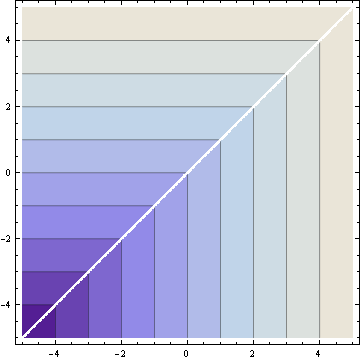
\includegraphics[width=2in]{./resources/hardmax.png}
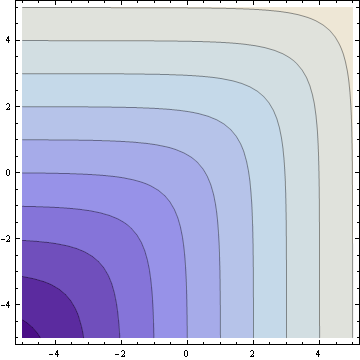
\includegraphics[width=2in]{./resources/softmax.png}
\end{center}
\end{figure}
\end{frame}

\begin{frame}
\frametitle{Multinomial Logit: Identification}
What is actually identified here?
\begin{itemize}
\item Helpful to look at the ratio of two choice probabilities
\begin{align*}
\frac{\sigma_{ij}(\theta)}{\sigma_{ik}(\theta)}  = \frac{e^{V_{ij}}}{e^{V_{ik}}} = e^{V_{ij} - V_{ik}}
\end{align*}
\item We only identify the \alert{difference in indirect utilities} not the levels.
\item The ratio of choice probabilities for $j$ and $k$ depends only on $j$ and $k$ and not on any alternative $l$, this is known as \alert{independence of irrelevant alternatives}.
\item For some (Luce (1959)) IIA was an attractive property for axiomatizing choice. (A feature or a bug?)
\item In fact the logit was derived in the search for a statistical model that satsified various axioms.
\end{itemize}
\end{frame}

\begin{frame}
\frametitle{Multinomial Logit: Identification}
As another idea suppose we add a constant $C$ to each $\beta_j$.
\begin{eqnarray*}
\sigma_{ij} = \frac{\exp[\symbf{x_i} (\beta_j+C) ]}{\sum_k \exp[\symbf{x_i} (\beta_k+C) ]} =  \frac{\exp[\symbf{x_i} C] \exp[\symbf{x_i} \beta_j ]}{\exp[\symbf{x_i} C] \sum_k \exp[\symbf{x_i} \beta_k ]}
\end{eqnarray*}
This has no effect.  That means we need to fix a normalization $C$.\\
 The most convenient is generally that $C = - \beta_K$.
\begin{itemize}
\item We normalize one of the choices to provide a utility of zero.
\item We actually already made another normalization. Does anyone know which?
\end{itemize}
\end{frame}


\begin{frame}
\frametitle{Multinomial Logit: Identification}
The most sensible normalization in demand settings is to allow for an \alert{outside option} which produces no utility in expectation so that $e^{V_{i0}} = e^{0}=1$:
\begin{eqnarray*}
\sigma_{ij} = \frac{e^{V_{ij} }}{1+\sum_k e^{V_{ik} }}
\end{eqnarray*}
\begin{itemize}
\item Hopefully the choice of outside option is well defined: not buying a yogurt, buying some other used car, etc.
\item Now this resembles the binomial logit model more closely.
\end{itemize}
\end{frame}


\begin{frame}{Back to Scale of Utility}
\begin{itemize}
\item For the logit, $U_{ij}^{*} = V_{ij} + \varepsilon_{ij}^{*}$ has $Var(\varepsilon^{*}) = a^2 \pi^2/6$; dividing by the scale parameter $a$ gives $U_{ij} = V_{ij}/a + \varepsilon_{ij}$ and $Var(\varepsilon) = \pi^2/6$
\begin{eqnarray*}
\sigma_{ij} = \frac{e^{V_{ij}/a}}{\sum_k e^{V_{ik}/a}} \approx \frac{e^{\beta^{*}/a \cdot x_{ij}}}{\sum_k e^{\beta^{*}/a \cdot x_{ik}}}
\end{eqnarray*}
\item Every coefficient $\beta$ is rescaled by $a$. This implies that only the ratio $\beta^{*}/a$ is identified.
\item Coefficients are relative to variance of unobserved factors. More unobserved variance $\longrightarrow$ smaller $\beta$.
\item Ratio $\beta_1/\beta_2$ is invariant to the scale parameter $a$. (\alert{marginal rate of substitution}).
\end{itemize}
\end{frame}


\begin{frame}{IIA Property}
The well known critique:
\begin{itemize}
\item You can choose to go to work on a car $c$ or blue bus $bb$. $\sigma_{c} = \sigma_{bb} = \frac{1}{2}$ so that $\frac{\sigma_c}{\sigma_{bb}} = 1$.
\item Now we introduce a red bus $rb$ that is identical to $bb$. Then $\frac{\sigma_{rb}}{\sigma_{bb}} = 1$ and $\sigma_{c} = \sigma_{bb}= \sigma_{rb} = \frac{1}{3}$ as the logit model predicts.
\item In reality we don't expect painting a bus red would change the number of individuals who drive a car so we would anticipate $\sigma_{c} = \frac{1}{2}$ and $\sigma_{bb} = \sigma_{rb} = \frac{1}{4}$.
\item We may not encounter too many cases where $\rho_{\varepsilon_{ik},\varepsilon_{ij}} \approx 1$, but we have many cases where this $\rho_{\varepsilon_{ik},\varepsilon_{ij}} \neq 0$
\item What we need is the ratio of probabilities to change when we introduce a third option!
\end{itemize}
\end{frame}

\begin{frame}{IIA Property}
\begin{itemize}
\item IIA implies that we can obtain consistent estimates for $\beta$ on any subset of alternatives.
\item This means instead of using all $\calJ$ alternatives in the choice set, we could estimate on some subset $\calS \subset \calJ$.
\item This used to be a way to reduce the computational burden of estimation (not clear this is an issue in 21st century).
\item Sometimes we have \alert{choice based samples} where we oversample people who choose a particular alternative. Manski and Lerman (1977) show we can get consistent estimates for all but the ASC. This requires knowledge of the difference between the true (population) rate $A_j$ and the choice-based sample rate $H_j$.
\item Hausman proposes a specification test of the logit model: estimate on the full dataset to get $\hat{\beta}$, construct a smaller subsample $\calS^k \subset \calJ$ and $\hat{\beta^k}$ for one or more subsets $k$. If $|\hat{\beta}^k - \hat{\beta}|$ is small enough.
\end{itemize}
\end{frame}

\begin{frame}
\frametitle{Own and Cross Elasticity}
\footnotesize
For the linear $V_{ij}$ case we have that $\frac{\partial V_{ij}}{\partial z_{ij}}=  \beta_z$.
\begin{eqnarray*}
\frac{\partial \sigma_{ij}}{\partial z_{ij}} &=& \sigma_{ij}(1- \sigma_{ij}) \frac{\partial V_{ij}}{\partial z_{ij}}\\
\text{ And Elasticity: }\quad  \frac{ \partial \log \sigma_{ij}}{ \partial \log z_{ij}} &=& \sigma_{ij}(1- \sigma_{ij}) \frac{\partial V_{ij}}{\partial z_{ij}} \frac{z_{ij}}{\sigma_{ij}} = (1- \sigma_{ij}) z_{ij} \frac{\partial V_{ij}}{\partial z_{ij}}\\
\text{ With cross effects: }\quad \frac{\partial \sigma_{ij}}{\partial z_{ik}} &=& -\sigma_{ij} \sigma_{ik} \frac{\partial V_{ik}}{\partial z_{ik}}\\
\text{ and elasticity: }\quad \frac{ \partial \log \sigma_{ij}}{ \partial \log z_{ik}} &=& -\sigma_{ik} z_{ik} \frac{\partial V_{ik}}{\partial z_{ik}}
\end{eqnarray*}
\begin{itemize}
\item This implies that $ \eta_{jj} = \frac{\partial \sigma_{ij}}{\partial p_j} \frac{p_j}{\sigma_{ij}}  = \beta_p \cdot p_j \cdot (1-\sigma_{ij})$.
\item The price elasticity is increasing in own price! (Why is this a bad idea?)
\item Also mechanical relationship between elasticity and \alert{share} so that popular products necessarily have higher markups (holding fixed prices).
\end{itemize}
\end{frame}



\begin{frame}{Proportional Substitution and Diversion}
Cross elasticity doesn't really depend on $j$:
\begin{eqnarray*}
\frac{ \partial \log \sigma_{ij}}{ \partial \log z_{ik}} = -\sigma_{ik} z_{ik} \underbrace{\frac{\partial V_{ik}}{\partial z_{ik}}}_{\beta_z}.
\end{eqnarray*}
Recall the diversion ratio:
\begin{align*}
D_{jk} =\frac{\frac{\partial \sigma_{ik}}{\partial p_{j}}}{\left |\frac{\partial \sigma_{ij}}{\partial p_{j}} \right|} = \frac{\beta_p \sigma_{ik} \sigma_{ij}}{\beta_p \sigma_{ij} (1-\sigma_{ij})} = \frac{\sigma_{ik}}{1-\sigma_{ij}}
\end{align*}
\begin{itemize}
\item This leads to the idea of \alert{proportional substitution}. As option $k$ gets better it proportionally reduces the shares of the all other choices.
\item Likewise removing an option $j$ means that $\tilde{\sigma}_{ik}(\calJ \setminus j) = \frac{\sigma_{ik}}{1-\sigma_{ij}}$ for all other $k$.
\item IIA/Logit means \alert{constant diversion ratios}. This might be a desirable property but probably not.
\end{itemize}
\end{frame}


\begin{frame}
\frametitle{Welfare: Consumer Surplus from the Inclusive Value}
With utility linear in price, $V_{ij} = v_{ij} - \alpha p_j$, $\alpha$ is the marginal utility of income and (Small and Rosen 1981):
\begin{eqnarray*}
\E[CS_i] = \frac{1}{\alpha} \log \left( \sum_{k \in \calJ} \exp[V_{ik}] \right) + C
\end{eqnarray*}
For any counterfactual (price change, new product, removal) the constant $C$ differences out:
\begin{eqnarray*}
\Delta CS_i = \frac{1}{\alpha}\left[ \log \left(\sum_{k \in \calJ^{1}} \exp[V_{ik}^{1}]\right)- \log \left( \sum_{k \in \calJ^{0}} \exp[V_{ik}^{0}] \right)\right]
\end{eqnarray*}
\begin{itemize}
\item Constant $\alpha$ means \alert{no income effects}: $CV = EV = \Delta CS$.
\item With a random $\alpha_i$ (mixed logit) the $\frac{1}{\alpha_i}$ belongs inside the expectation over types and the clean closed form disappears (more next week).
\end{itemize}
\end{frame}

\begin{frame}
\frametitle{Worked Example: The Welfare Cost of Removing a Product}
Three inside goods with $V_i = (1,\, 0.5,\, 0.5)$, outside good $V_{i0}=0$, and $\alpha = 1$ (so utils are dollars):
\begin{eqnarray*}
\Delta CS_i = \frac{1}{\alpha}\left[\log (\underbrace{1 + e^{0.5} + e^{0.5}}_{= 4.30}) - \log (\underbrace{1 + e^{1} + e^{0.5}+ e^{0.5}}_{= 7.02}) \right] = -0.49
\end{eqnarray*}
\begin{itemize}
\item For logit this collapses to $\Delta CS_i = \frac{1}{\alpha} \log(1-\sigma_{ij})$: the welfare cost of removing $j$ depends \alert{only on its share} ($\sigma_{i1} = 0.39$ here) --- IIA strikes again.
\item This is Hausman (1997)'s Apple-Cinnamon Cheerios question. In product space he had to find a \alert{virtual (choke) price} $p_j^{*}$ that zeroes out demand; in discrete choice we just drop $j$ from $\calJ$ and the log-sum-exp does the rest.
\item Same object as $WTP_i(j)$: reappears in HW2 and for hospital networks (Capps, Dranove, Satterthwaite 2003) later in the course.
\item Caveat: full-support $\varepsilon_{ij}$ means \alert{every} new product mechanically adds surplus (new-goods bias: Petrin 2002; more in the micro data lecture).
\end{itemize}
\end{frame}

\begin{frame}
\frametitle{CES and Logit: Two Sides of the Same Coin}
Recall the CES verdict from last week: one elasticity, one markup, ``hard to do IO here.'' Look familiar?
\begin{center}
\small
\begin{tabular}{lcc}
& CES & Logit \\
\midrule
Own elasticity & $-\sigma$ (same for all goods) & $-\alpha p_j (1-\sigma_{ij}) \approx -\alpha p_j$ \\
Substitution & proportional to expenditure share & proportional to share (IIA) \\
Markup & $p = mc/\rho$ (same for all goods) & $p_j - mc_j = \frac{1}{\alpha(1-\sigma_{ij})}$ \\
\end{tabular}
\end{center}
\begin{itemize}
\item Anderson, de Palma, Thisse (1992): a CES representative consumer and a population of logit consumers generate the \alert{same} aggregate demand system (CES is homothetic with continuous quantities; logit is unit demand --- otherwise the same model).
\item The fixes rhyme too: nested logit $\leftrightarrow$ nested CES; mixed logit $\leftrightarrow$ random-coefficients CES (both workhorses in Trade and Macro).
\item IO speaks discrete choice because we want product-level $(p_{jt}, x_{jt}, \xi_{jt})$ --- but the pathologies and their cures translate across languages.
\end{itemize}
\end{frame}


\section{Thanks!}

\end{document}
